\documentclass[a4paper, 12pt]{article}

\usepackage{cmap}
\usepackage{mathtext} 
\usepackage[T2A]{fontenc}
\usepackage[utf8]{inputenc}
\usepackage[english,russian]{babel}

\usepackage{amsfonts,amssymb,amsthm,mathtools}
\usepackage{amsmath}
\usepackage{icomma} 

\usepackage{graphicx} 
\graphicspath{{Picturies/}}
\usepackage{wrapfig}

\usepackage{array,tabularx,tabulary,booktabs}
\usepackage{longtable}
\usepackage{multirow}

\usepackage{caption}
\usepackage{subcaption}
\captionsetup{labelsep=period}

\renewcommand{\phi}{\varphi}
\newcommand{\eps}{\varepsilon}
\renewcommand{\AA}{\ensuremath{\mathring{A}}}
\newcommand{\parag}[1]{\paragraph*{#1:}}

\newcounter{Points}
\setcounter{Points}{1}
\newcommand{\point}{\arabic{Points}. \addtocounter{Points}{1}}

\author{Вязовцев Андрей, Б01-005}
\date{11.03.22}
\title{Лабораторная работа 4.7.2. Эффект Поккельса.}

\begin {document}

\maketitle

\parag {Цель работы} исследовать интерференцию рассеянного света, прошедшего кристалл; наблюдать изменение характера поляризации света при наложении на кристалл электрического поля.

\parag {В работе используются} гелий-неоновый лазер, поляризатор, кристалл ниобата лития, матовая пластинка, экран, источник высоковольтного переменного и постоянного напряжения, фотодиод, осциллограф, линейка.

\parag {Теоретическая справка} ~\\

Выражение для радиуса кольца имеет вид:

\begin{equation}
    r^2_m = \frac{\lambda}{l} \frac{(n_o L)^2}{(n_o - n_e)} m
    \label{eq:radius} 
\end{equation}

Где $n_o$ --- показатель преломления для векторов $\vec{E}$, перпендикулярных главной оптической оси $Z$ (обыкновенная, ординарная волна), а $n_e$ --- параллельных $Z$ (необыкновенная, экстраординарная волна). Величина $n_o - n_e$ называется двулучепреломлением кристалла. 

\parag {Экспериментальная установка} ~

Схему рабочего места можно посмотреть на рис. \ref{img:workplace}.

\begin{figure}[!h]
    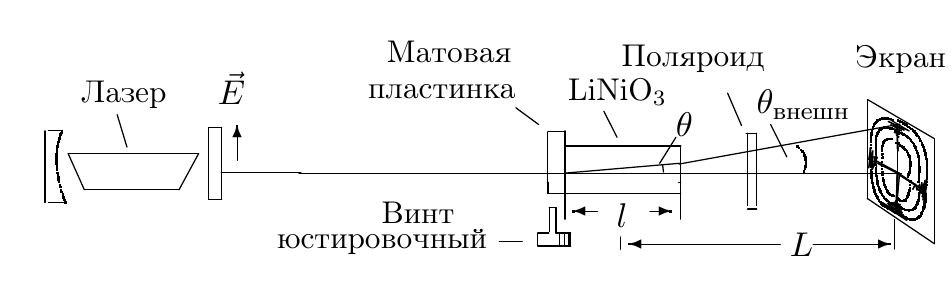
\includegraphics[scale = 0.4]{Workplace}
    \centering
    \caption{Схема для наблюдения интеренференционной картины}
    \label{img:workplace}
\end{figure}

\parag {Ход работы} ~\\

\point Соберем оптическую схему согласно рис. \ref{img:workplace}. Убедимся, что лазер поляризован вертикально. Установим кристалл. Получим на экране интеренференционную картину. Поставим анализатор в положении горизонтального разрешённого направления.

\point Измерим радиусы тёмных колец $r(m)$ и расстояние $L$ от середины кристалла до экрана. Получаем: $L = 73,5$ см. 

\begin{table}[!h]
    \centering
    \begin{tabular}{|c|c|c|c|c|c|c|c|c|}
        \hline
        $m$ & 1 & 2 & 3 & 4 & 5 & 6\\ \hline
        $r$, мм & 27 & 37 & 45 & 52 & 59 & 67\\ \hline
        $r^2$, $мм^2$ & 729 & 1369 & 2025 & 2704 & 3481 & 4489 \\ \hline
    \end{tabular}
    \caption {Радиусы тёмных колец}
    \label{table:light}
\end{table}

Построим график $r^2 = f(m)$. Результаты см. на рис. \ref{img:graph}.

\begin{figure}[!b]
    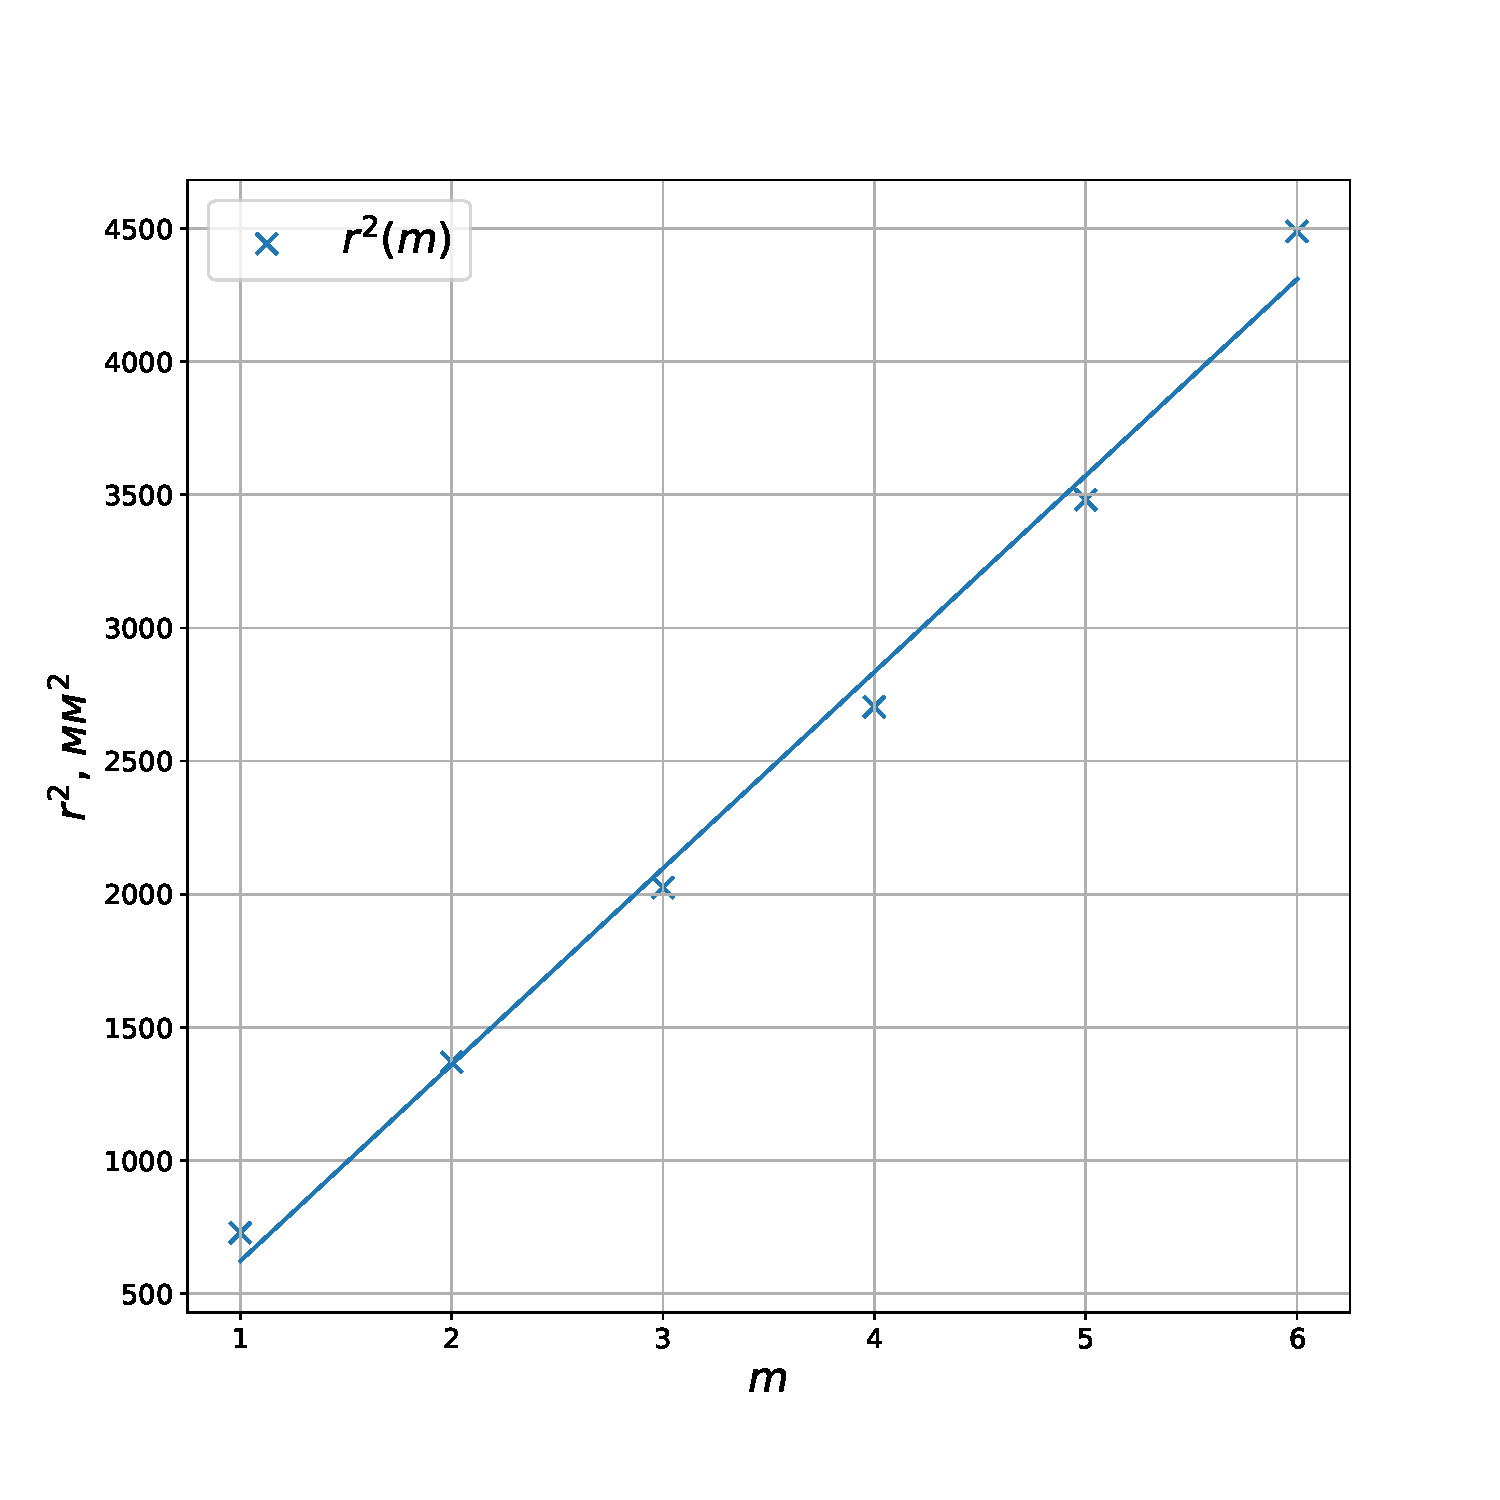
\includegraphics[scale = 0.5]{graph}
    \centering
    \caption{График зависимости $r^2 (m)$}
    \label{img:graph}
\end{figure}

С помощью формулы \eqref{eq:radius} и графика найдём двулучепреломление кристалл ниобата лития. Т.~к. 

\begin{align*}
    \frac{r^2}{m} &= (730 \pm 30) ~мм^2 \\
    l &= 26~мм \\
    \lambda &= 630~нм \\
    n_o &= 2.29
\end{align*}

то получаем:

\[
    n_o - n_e = (9,4 \pm 0,4) \cdot 10^{-2}
\]

\point Уберём матовую пластинку, подключим блок питания в режиме постоянного напряжения. Определим полуволновое напряжение $U_\frac{\lambda}{2}$. Получаем:

\[
    U_\frac{\lambda}{2} = 30 дел. = 450~В
\]

\point Убедимся, что при $U_\frac{\lambda}{4} = \dfrac{1}{2} U_\frac{\lambda}{2}$ поляризация носит круговой характер.

\point Установим вместо экрана фотодиод, напряжение поменяем на переменное, подключим осциллограф.

\point Измерим с помощью фигур Лиссажу полуволновое напряжение. Получаем:

\[
    U_\frac{\lambda}{2} = \Delta U \approx 636~В
\]

\point Запечатлим фигуры Лиссажу для различных напряжений при скрещенных поляризациях лазера и анализатора.

Заметим, что при смене поляризации на параллельную картина <<переворачивается>>.

\begin{figure}[!h]

\begin{subfigure}{0.5\textwidth}
    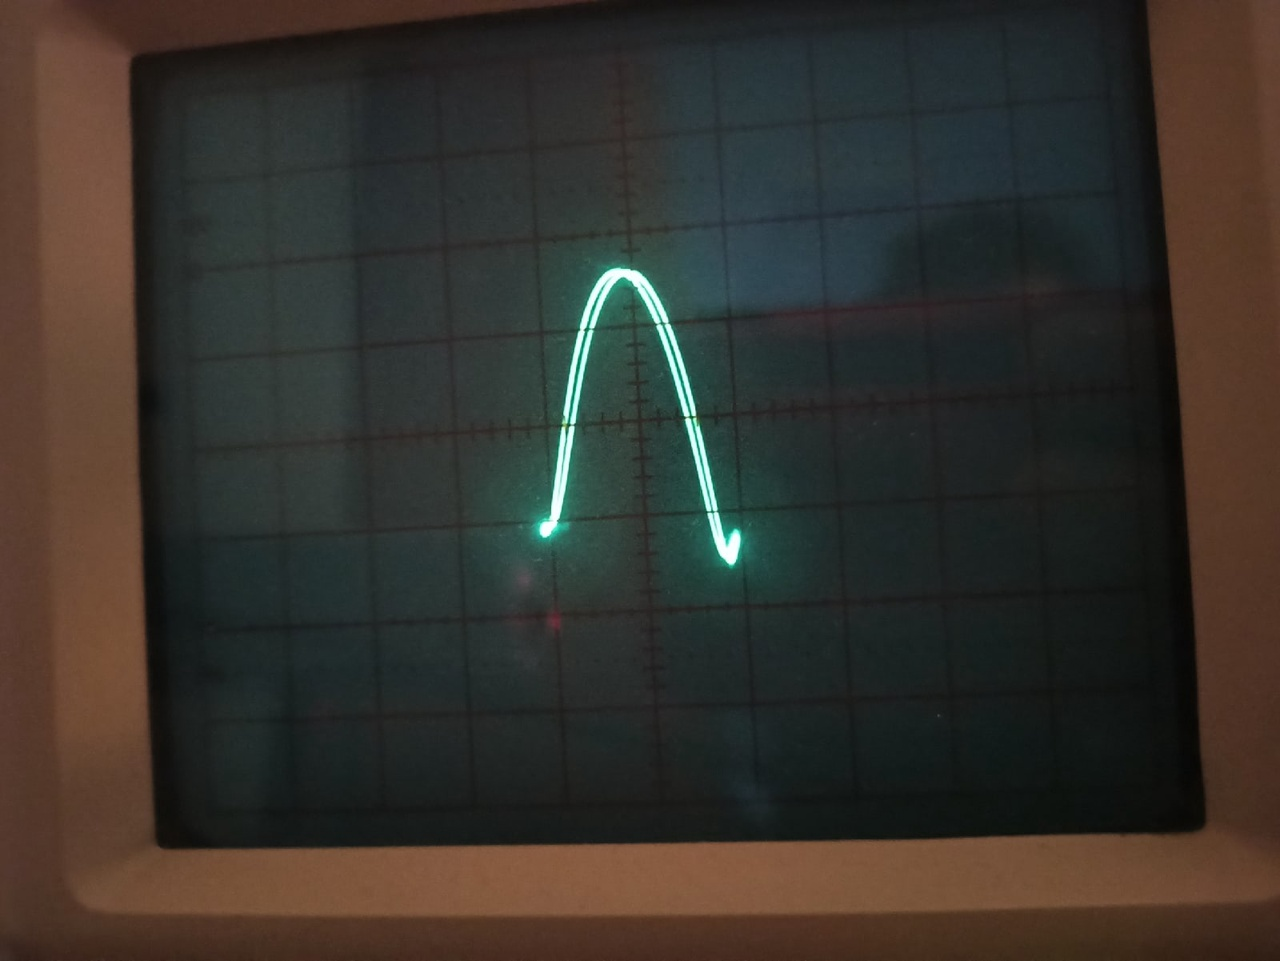
\includegraphics[scale = 0.15]{intersect1}
    \centering
    \caption{Скрещенная $U_\frac{\lambda}{2}$\\~}
\end{subfigure}
\begin{subfigure}{0.5\textwidth}
    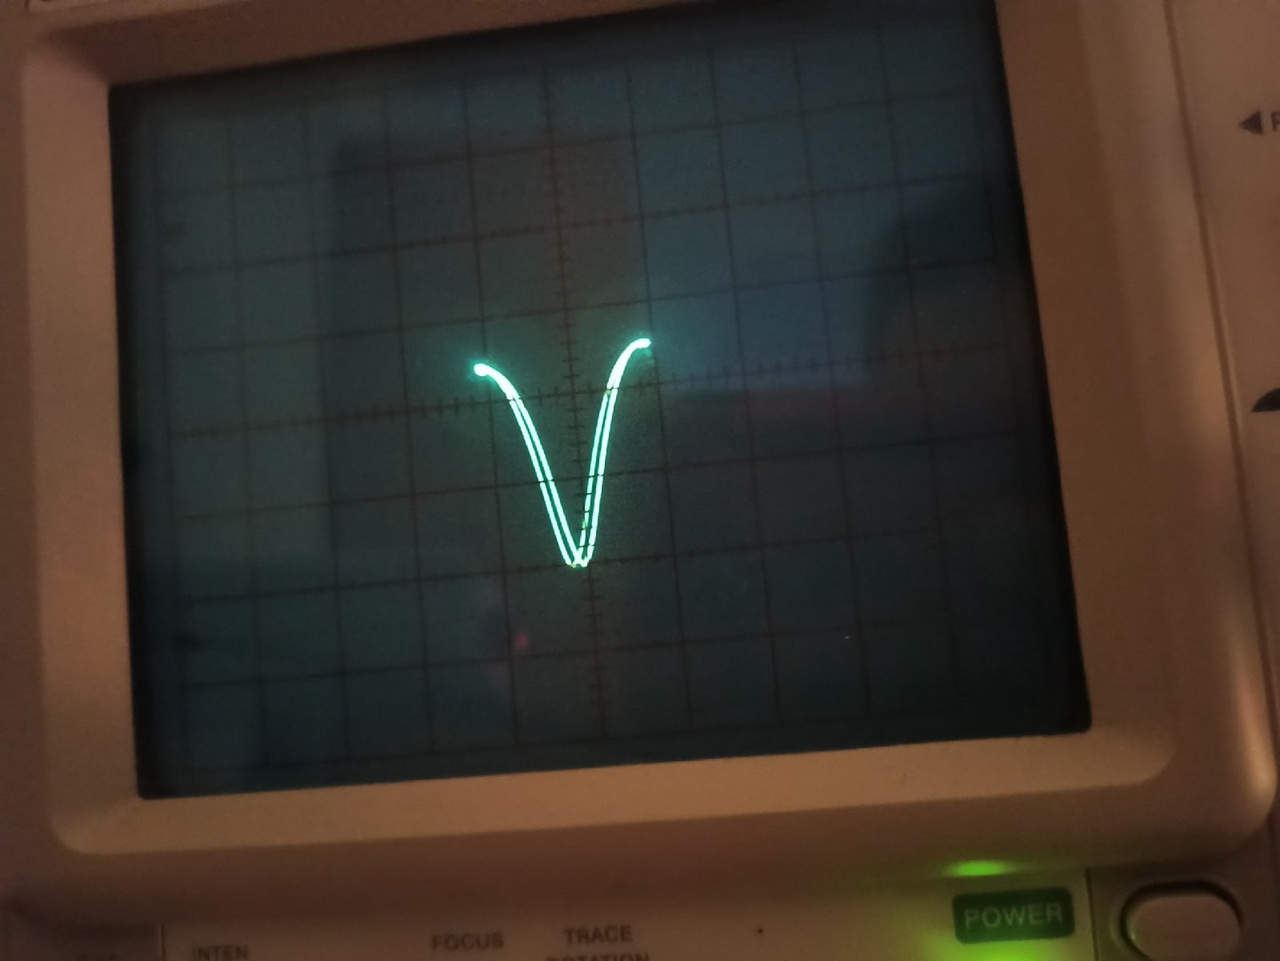
\includegraphics[scale = 0.15]{parallel1}
    \centering
    \caption{Параллельная $U_\frac{\lambda}{2}$\\~}
\end{subfigure}

\begin{subfigure}{0.5\textwidth}
    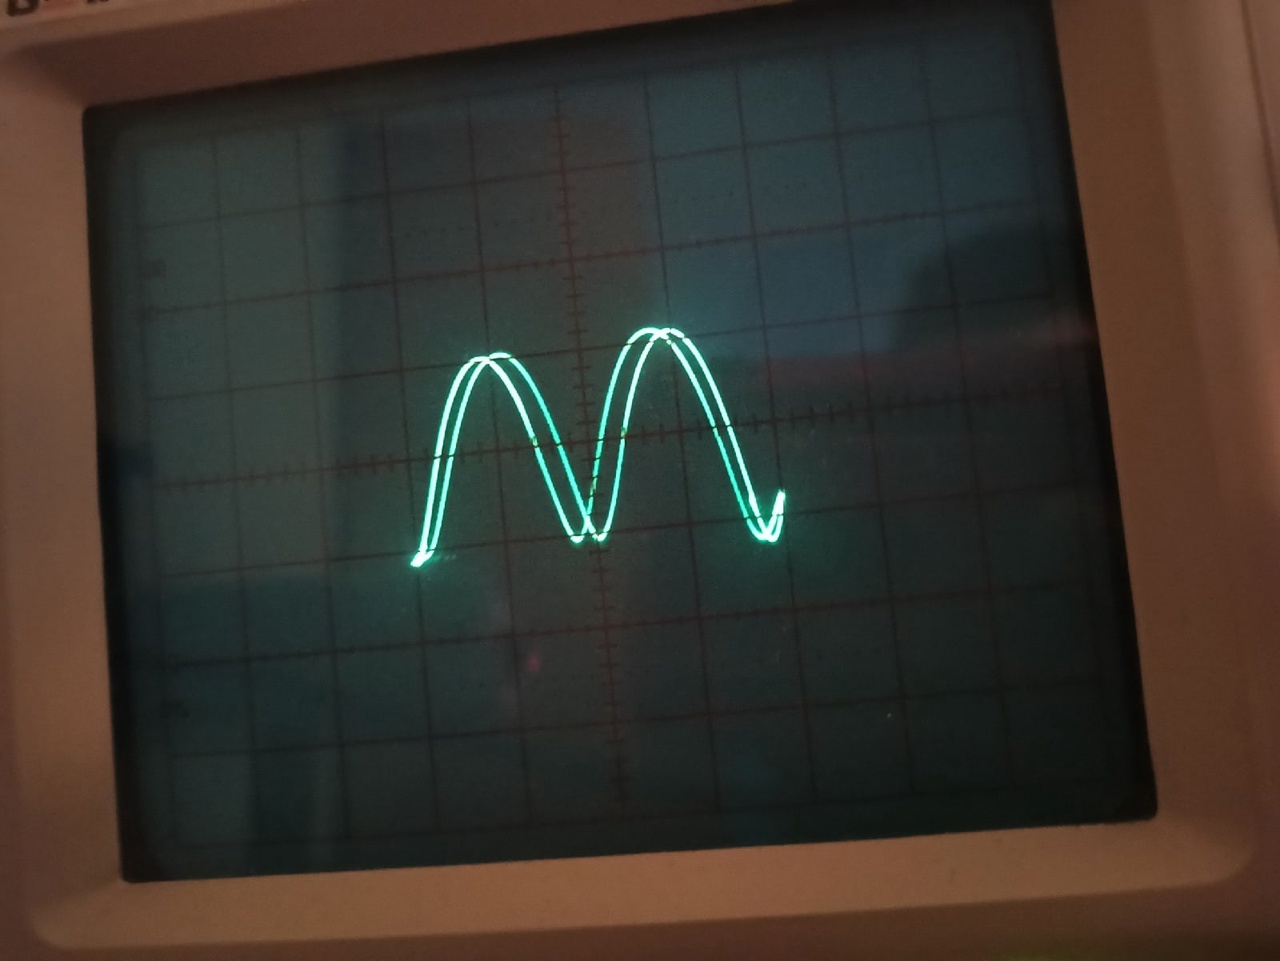
\includegraphics[scale = 0.15]{intersect2}
    \centering
    \caption{Скрещенная $U_\lambda$\\~}
\end{subfigure}
\begin{subfigure}{0.5\textwidth}
    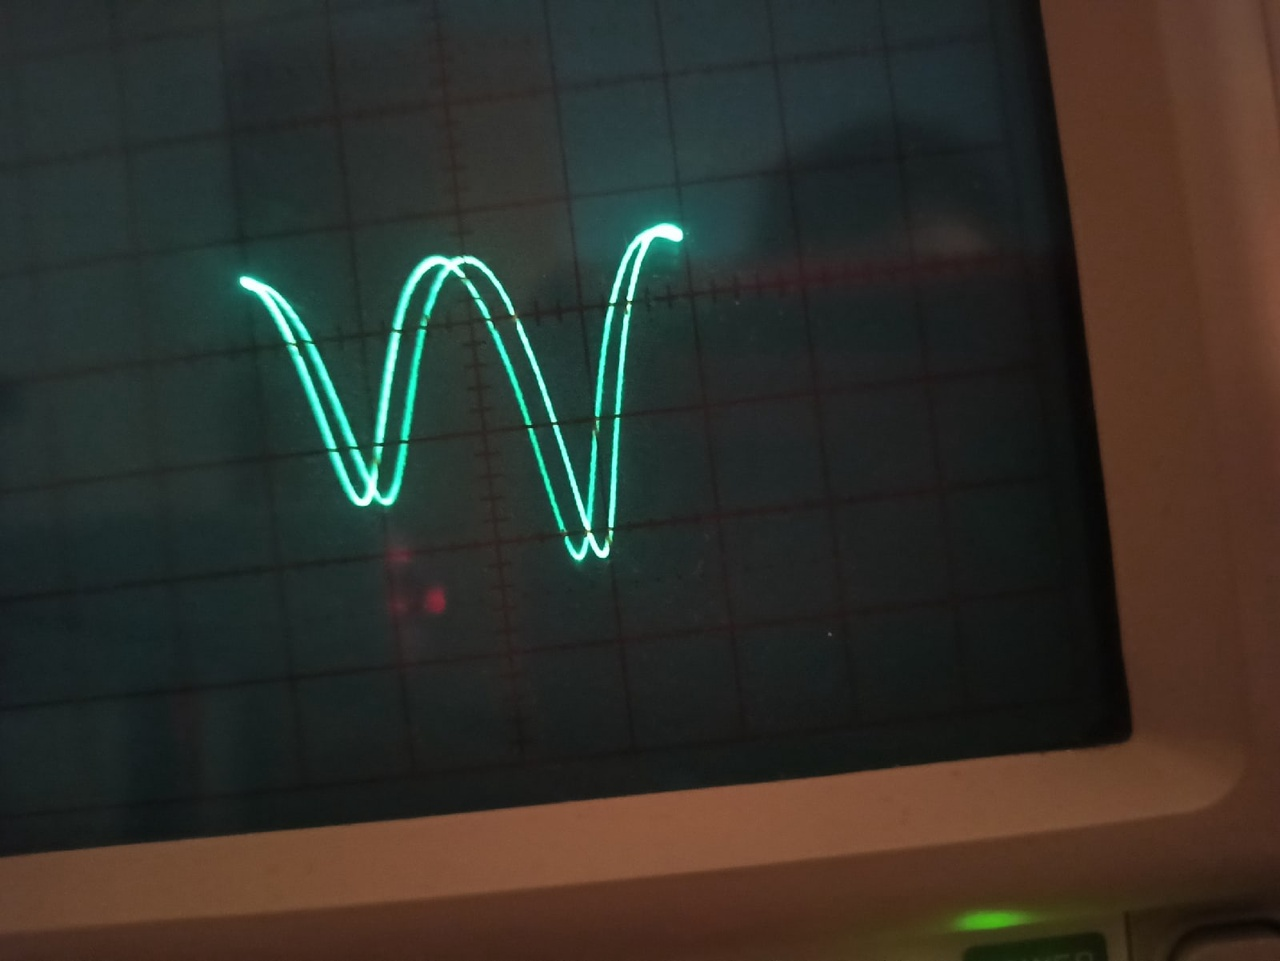
\includegraphics[scale = 0.15]{parallel2}
    \centering
    \caption{Параллельная $U_\lambda$\\~}
\end{subfigure}

\begin{subfigure}{0.5\textwidth}
    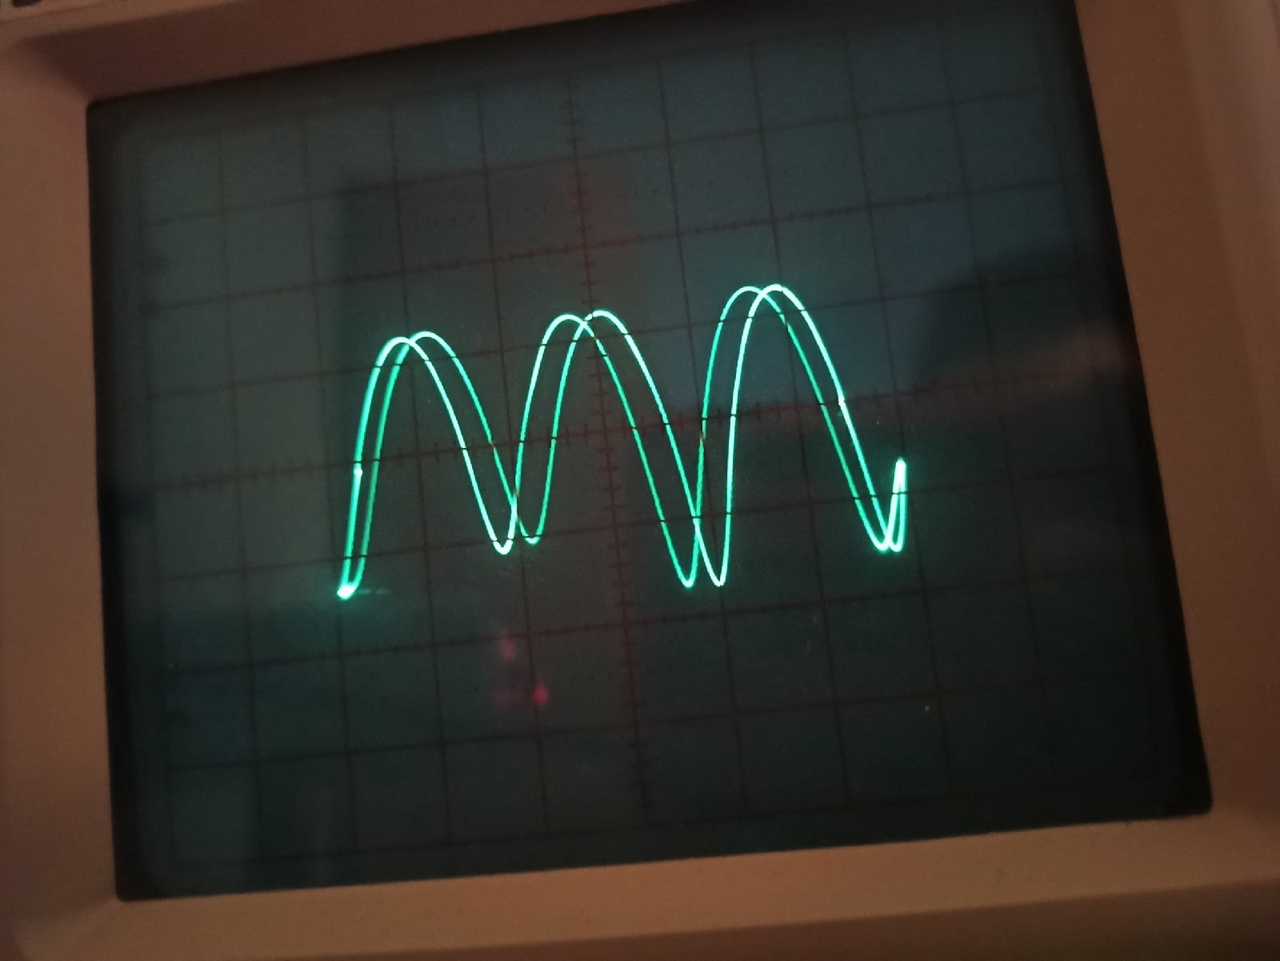
\includegraphics[scale = 0.15]{intersect3}
    \centering
    \caption{Скрещенная $U_\frac{3 \lambda}{2}$}
\end{subfigure}
\begin{subfigure}{0.5\textwidth}
    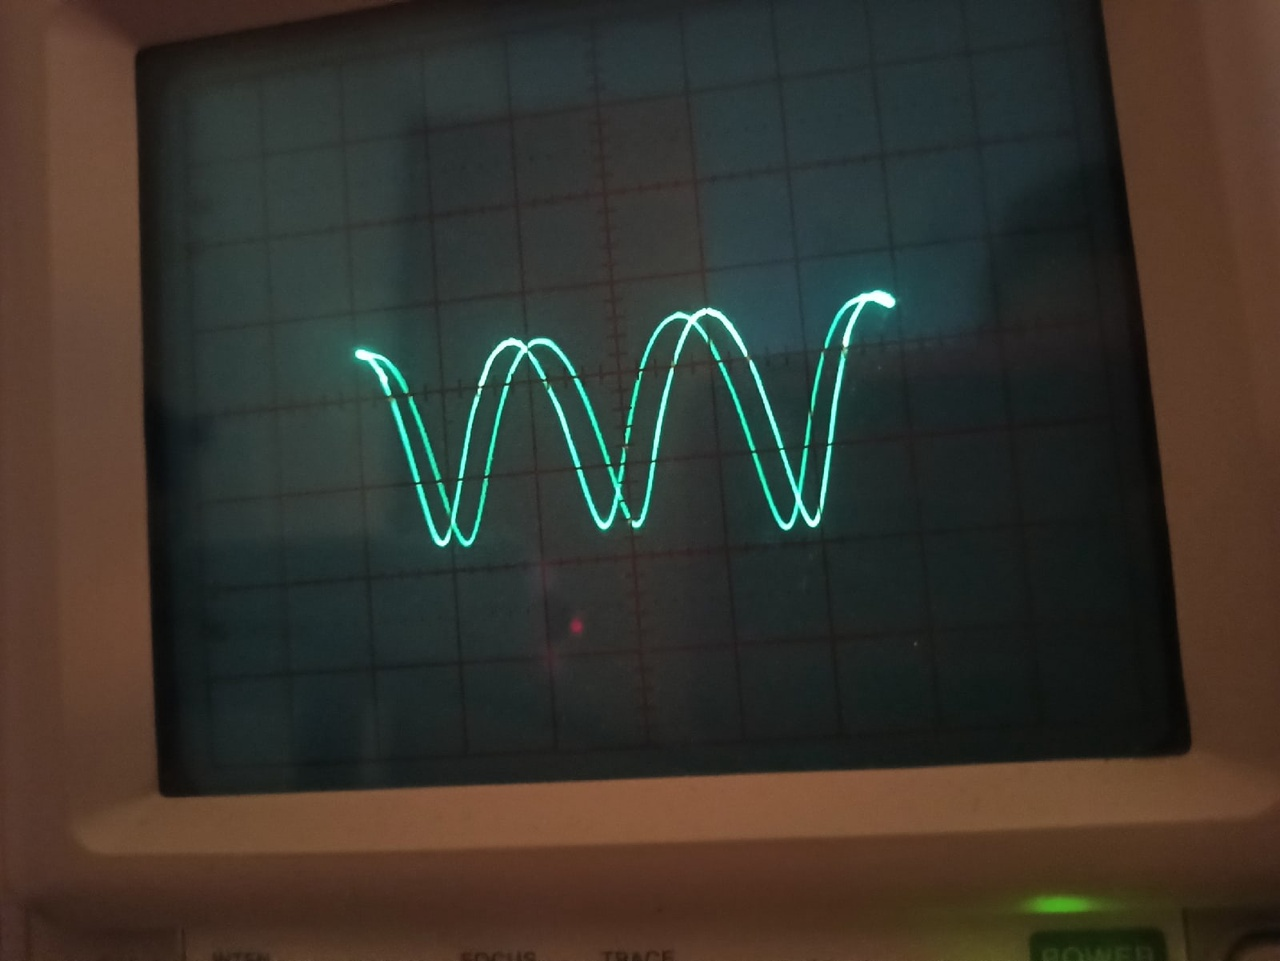
\includegraphics[scale = 0.15]{parallel3}
    \centering
    \caption{Параллельная $U_\frac{3 \lambda}{2}$}
\end{subfigure}

\end{figure}

\end {document}
